\section{Visual Programming}

The second part of this project is to develop a visual programming interface to program the robot
and improve the programming skills of the users. Since the hardware platform for this section has
been the same as for the trivial type game, hardware requirements are not included in this section.
Furthermore, since the same software design is followed for the communication with the robot, there
is no need on adding it to this section.

Therefore, here will be explained the software requirements for the visual programming client, the
design specification of the software that has been used for this section and the user manual for
this application, along with the issue management of this section, that will be mainly focused on
the software issues.

There is no need of explaining the testing plan, since it has been the same as the one used in the
trivial game, except from the real user testing, that there has not been an opportunity to do it.

\subsection{Software Requirements}

The software requirements of this application will be based on usability, minimal WebLab resource
usage and effectiveness of the programming. Those requirements are listed below:

\begin{itemize}

	\item The \acrlong{ui} must allow the user to understand how to program the robot.
	\item The \acrlong{ui} must show the robot doing what had been programmed to do.
	\item The robot must follow the code developed in the interface.
	\item The programming must not block the interface of the user.
	\item The program development must not use the resource until the test is reserved.
	\item The user must be able to edit the program after testing it.
	\item The server and the client must be loosely coupled.

\end{itemize}

Taking into account those requirements, it has been decided to develop a new experiment server and
to add some more \acrshort{api}s to WebLab client. Moreover, Google's Blockly~\cite{blockly} is
going to be used for the development, since it is the most known platform to create visual editors
in a web platform and contains code generators for \acrlong{js}, Dart~\cite{dart}, Python and
\acrshort{php}.

\subsection{Design Specification}

The software itself will follow the same design specification as in the trivial game. Nevertheless,
it has been decided that the code generation is going to be done in the client side, since it
supposes less security concern by using the \acrshort{api} provided by the experiment server and not
programming the experiment server itself (or even the robot). Therefore, \acrlong{js} generator will
be used.

Moreover, since one of the requirements is that the software must not use the resource (the robot
Romie) while the user is creating the program, and can only be reserved once the user tries to test
it, a new \acrshort{api} call is needed in the WebLab \acrlong{js} \acrshort{api}.

Moreover, since all commands in WebLab are sent asynchronously, the client must wait for the
movement to finish before attempting the next movement. The problem is that with a \emph{while}
loop, the interface would be broken in an infinite loop. In this case, and thanks to the advantages
brought by the scopes introduced by the \acrshort{js}-interpreter, the solution has been as simple
as creating some wrapper functions to move the robot. The real function example can be seen in
algorithm~\ref{alg:move_func}, the wrapper function example in algorythm~\ref{alg:wrapper} and the
generated code in algorithm~\ref{alg:generated}.

As it can be seen, the move functions are first defined in a similar way to what it was developed
for the trivial type game. Then, some wrappers are created for the functions and they are added to
the context of the code execution. That way, the block code can call those functions without
blocking the execution, enabling to insert a \emph{while} loop until the server responds.

\begin{center}
\begin{minipage}{.9\textwidth}
\singlespace
\fvset{frame=single}
\begin{pyglist}[language=javascript, caption={Robot movement function.},
	label={alg:move_func}, listingname={Algorithm}, numbers=left]
Romie = function() {
    this.moving = false;
}

Romie.prototype.forward = function() {
    this.moving = true;
    Weblab.sendCommand('{"command":"F"}', function(response) {
        this.moving = false;
    }.bind(this));
}

var romie = new Romie();
\end{pyglist}
\fvset{frame=none}
\end{minipage}
\end{center}

\begin{center}
\begin{minipage}{.9\textwidth}
\singlespace
\fvset{frame=single}
\begin{pyglist}[language=javascript, caption={Function wrapper.},
	label={alg:wrapper}, listingname={Algorithm}, numbers=left]
function initApi(interpreter, scope) {
	// Add Romie movement checker to the context
	var wrapper = function() {
		return interpreter.createPrimitive(romie.isMoving());
	};
	this.setProperty(scope, 'isMoving',
		this.createNativeFunction(wrapper));

	// Add an API function for the forward() block.
	wrapper = function() {
		romie.forward();
	};
	interpreter.setProperty(scope, 'forward',
		interpreter.createNativeFunction(wrapper));
}
var myInterpreter = new Interpreter(
	Blockly.JavaScript.workspaceToCode(workspace),
	initApi);
\end{pyglist}
\fvset{frame=none}
\end{minipage}
\end{center}

\begin{center}
\begin{minipage}{.9\textwidth}
\singlespace
\fvset{frame=single}
\begin{pyglist}[language=javascript, caption={Generated code.},
	label={alg:generated}, listingname={Algorithm}, numbers=left]
// Block code
Blockly.JavaScript['romie_move_forward'] = function(block) {
    code = 'forward();\n'+
            'while(isMoving());\n';
    return code;
};

// Which generates
forward();
while(isMoving());
\end{pyglist}
\fvset{frame=none}
\end{minipage}
\end{center}

Since one of the requirements is for the user to always know what is happening, the block
highlighting provided by Blockly will be used. This way, when the code is executed, the code being
executed will be highlighted, and the user can debug that code.

Furthermore, the \acrlong{ui} displays the two cameras of the robot once it starts testing the code.
This way, the user can see what is happening with the robot and actually test how the robot moves.
The complete experiment flow diagram is provided in figure~\ref{fig:blockly_flow}.

\begin{figure}[!htbp]
	\centering
	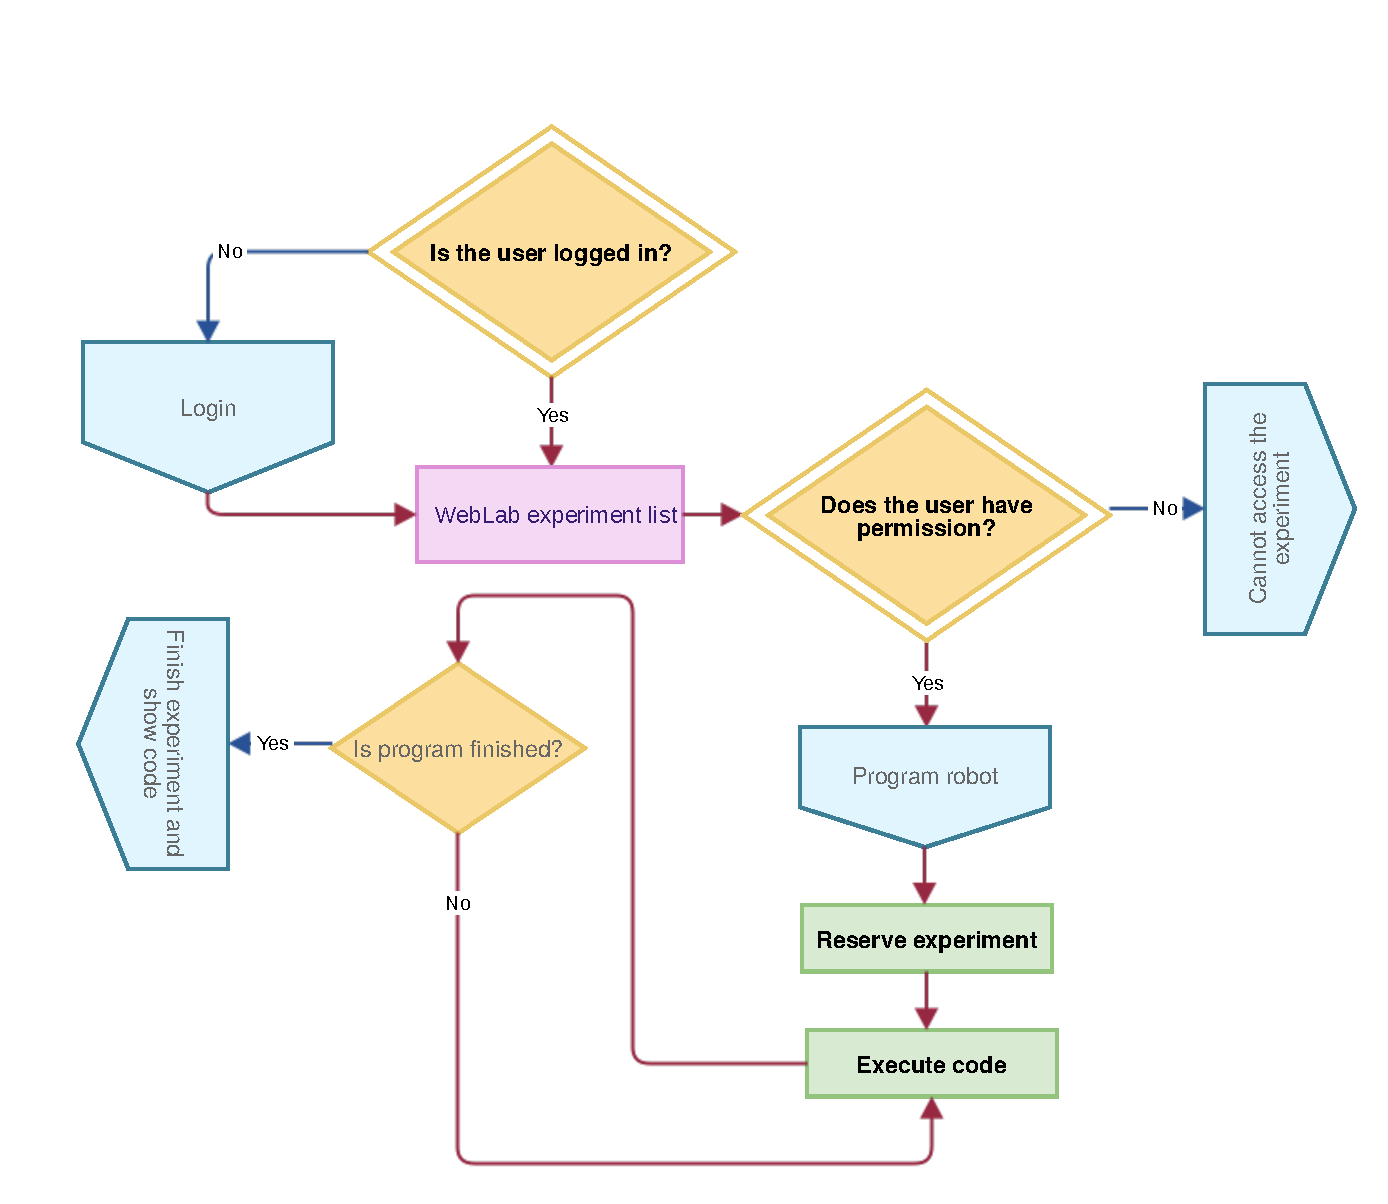
\includegraphics[width=0.85\textwidth]{fig/blockly-experiment-flow}
	\caption{Experiment flow for Romie's Blockly interface.}
	\label{fig:blockly_flow}
\end{figure}

\subsection{User Manual}

As in the case of the trivial type game, you must have an account in WebLab-Deusto and the
permission to use this experiment. You have to go to \url{https://weblab.deusto.es/weblab/client/}
and insert your credentials in the provided form.

Once logged in, you will see ``romie\_blockly'' experiment under the ``Robot experiments'' category.
You could see more experiments if you have the permission to use them. If you cannot find the
experiment you should contact the administrators. Click on ``romie\_blockly'' or in its image and
you will enter the programming page (figure~\ref{fig:man:blockly_reserve}).

\begin{figure}[!htbp]
	\centering
	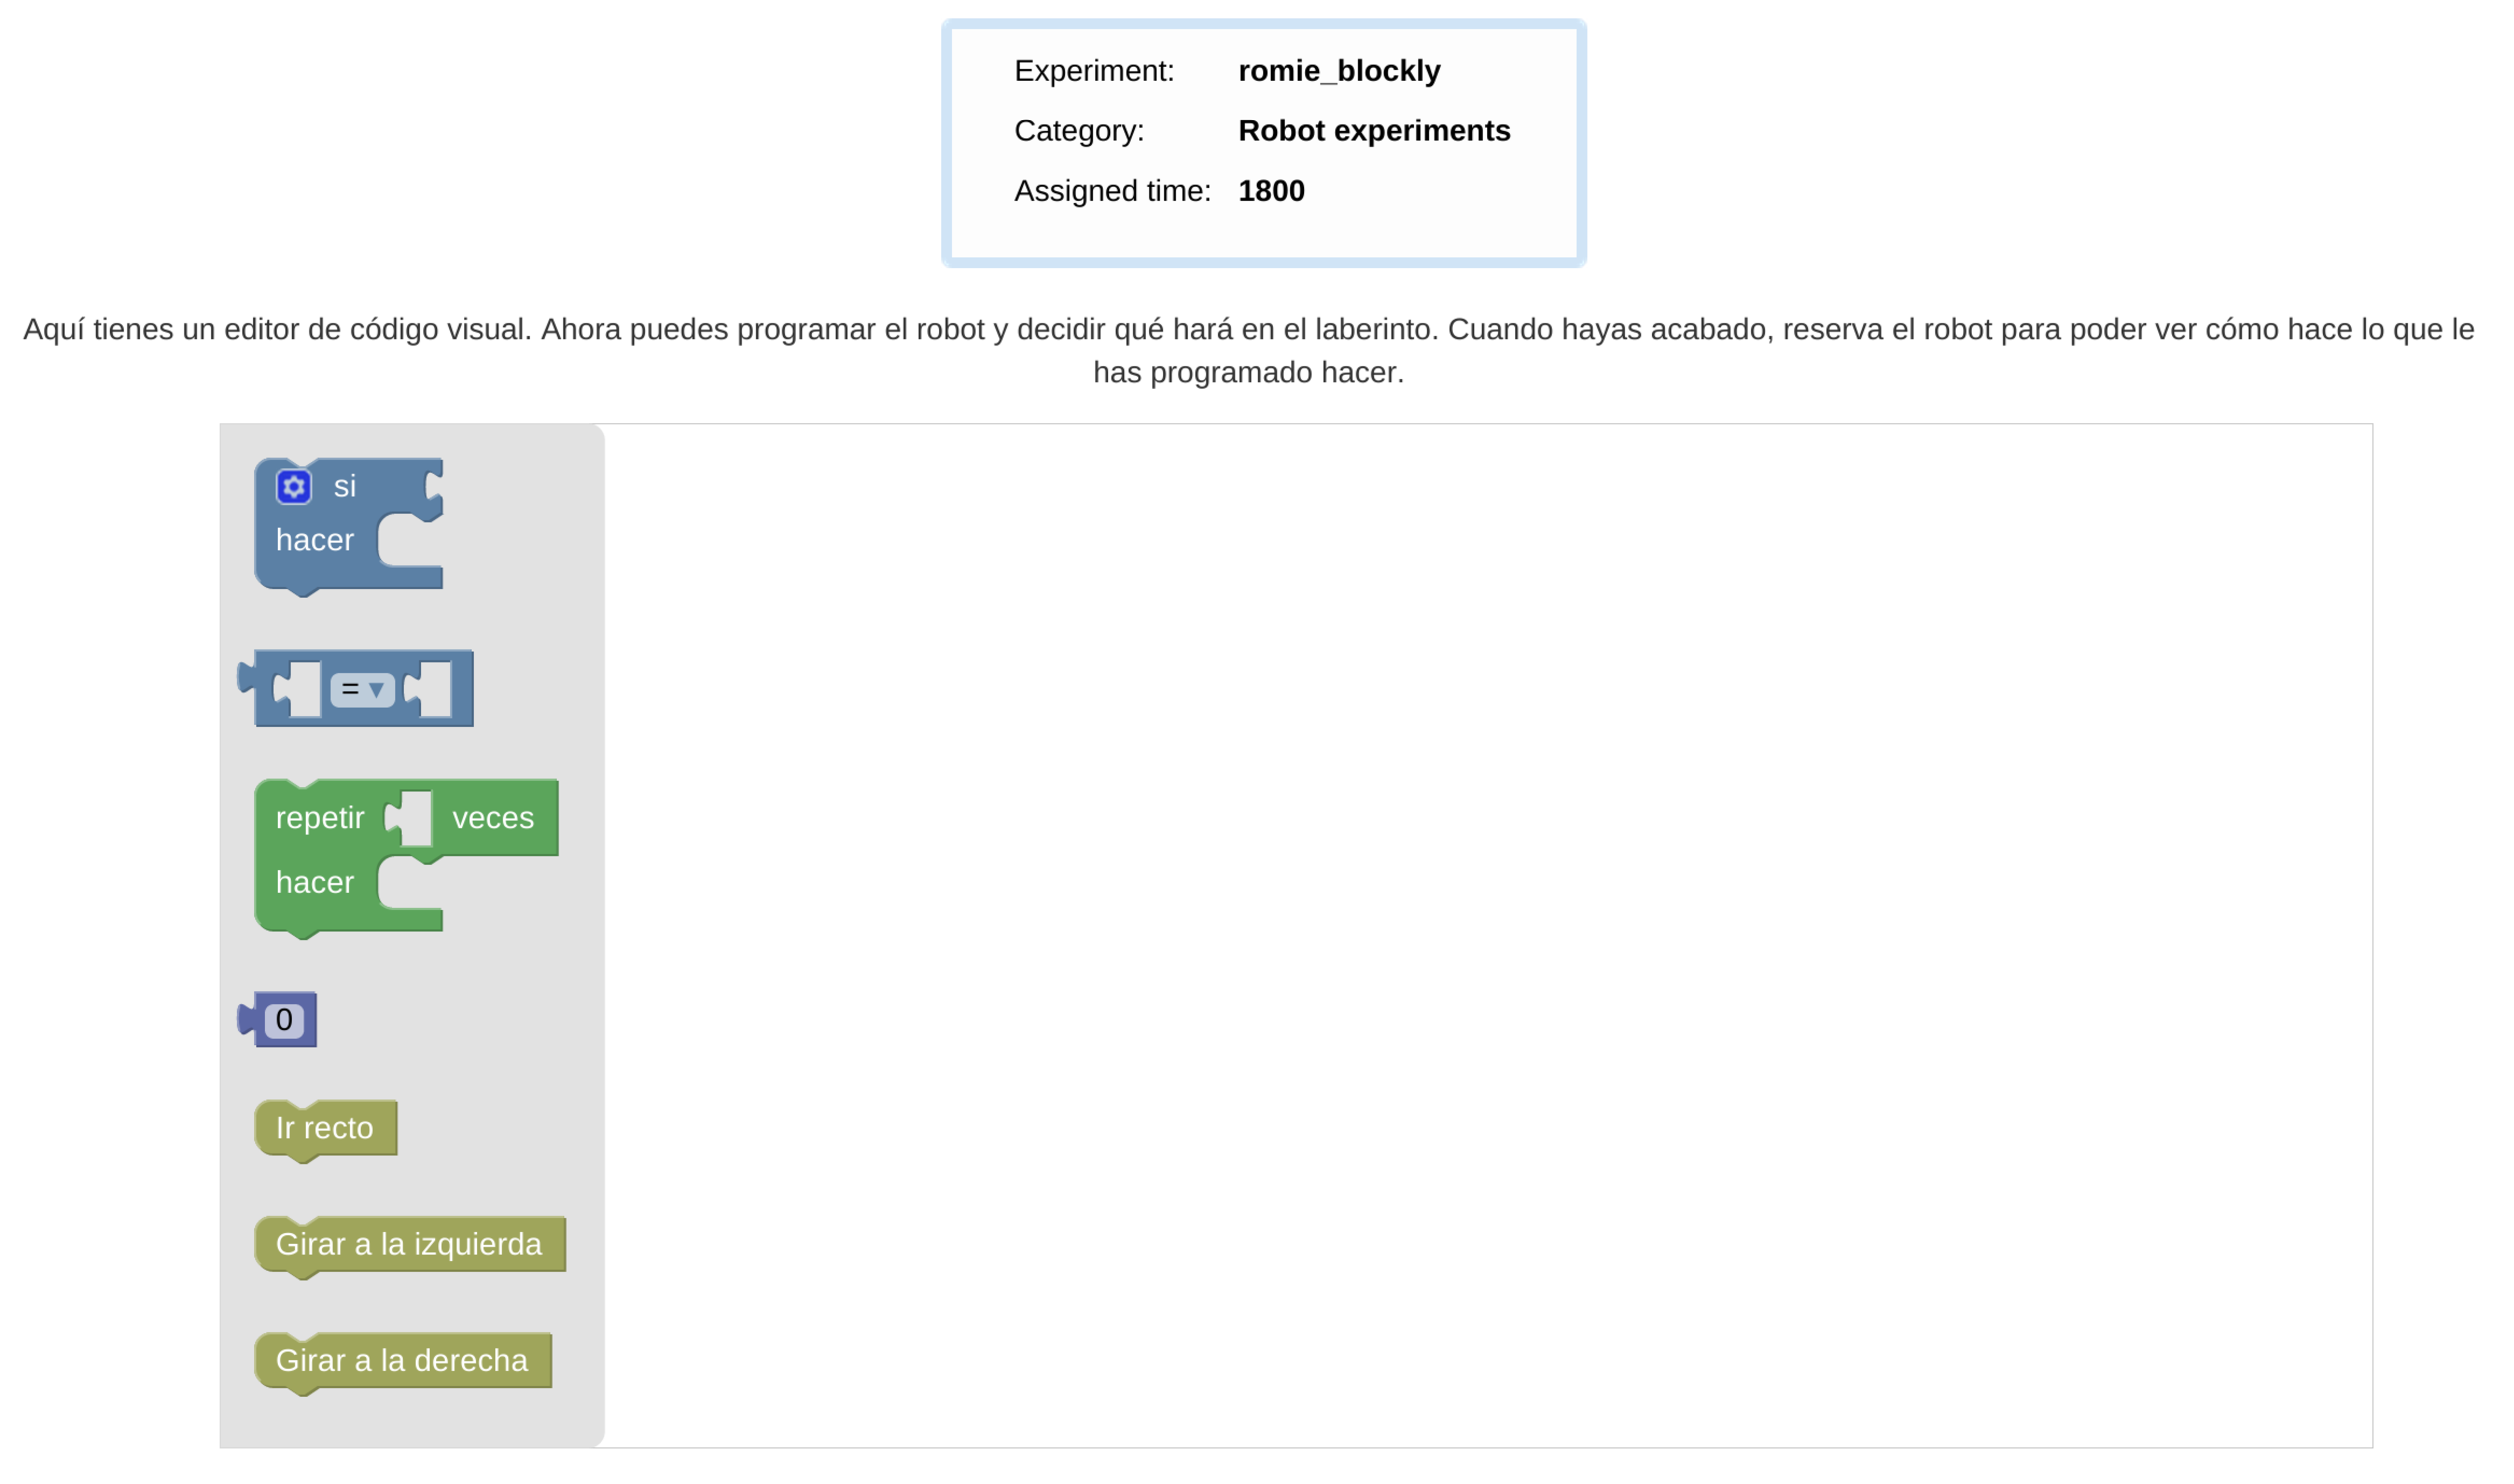
\includegraphics[width=0.85\textwidth]{fig/manuals/blockly/reservation}
	\caption{Writing code for Romie in WebLab-Deusto.}
	\label{fig:man:blockly_reserve}
\end{figure}

In this page, you will be able to program the robot. You will have some simple blocks that you can
use to create you would like to test. Once finished programming, you can press the ``Reserve''
button and reserve the experiment.

If somebody is using the experiment you will be put into queue. When you access the experiment, you
will see the code being executed in the left while you see the two cameras of the robot in the
right (figure~\ref{fig:man:blockly_playing}). You will be able to determine which piece of code is
being executed because it will be highlighted. Once the code finishes its execution, you will be
redirected to see your code. There you will be able to change the code and reserve the experiment
again.

\begin{figure}[!htbp]
	\centering
	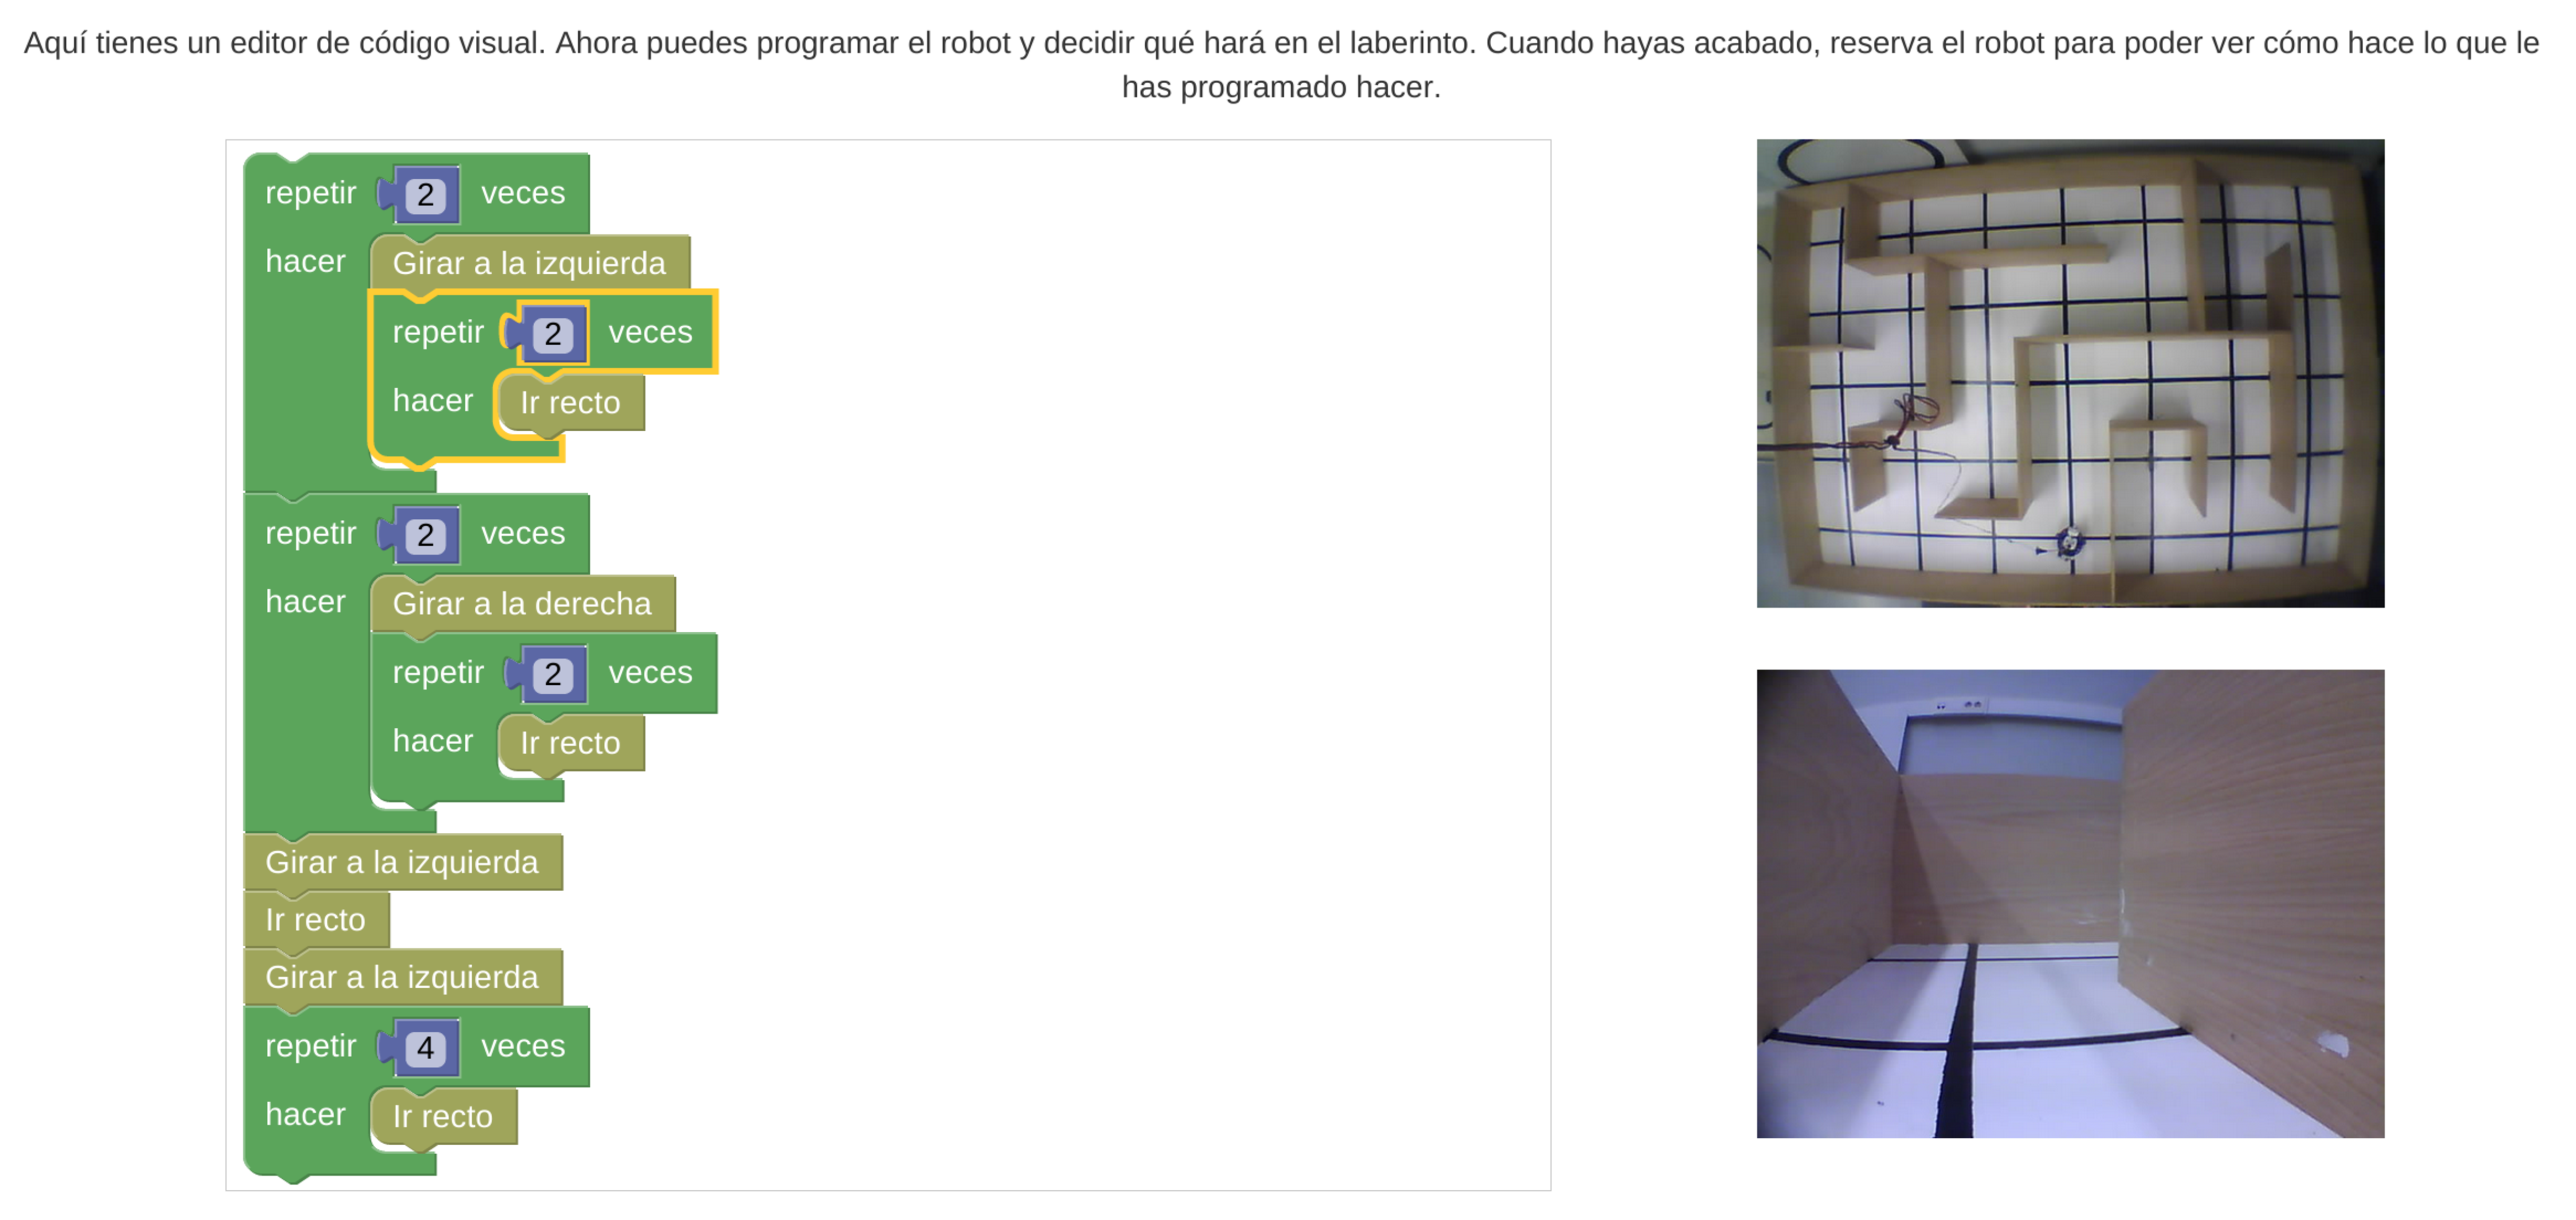
\includegraphics[width=0.85\textwidth]{fig/manuals/blockly/executing}
	\caption{Testing your code with Romie.}
	\label{fig:man:blockly_playing}
\end{figure}

\FloatBarrier

\subsection{Issue Management}

During the development of this scenario some issues have appeared and have been solved. The first of
them was that the \acrshort{api} of WebLab-Deusto was asynchronous, while in Blockly, for simple
tasks like moving forward, right, left, or checking sensors next commands had to wait for the
previous ones. This was solved using the contexts and wrappers for the functions that have been
explained before, in algorithm~\ref{alg:wrapper}.

\begin{center}
\begin{minipage}{.9\textwidth}
\singlespace
\fvset{frame=single}
\begin{pyglist}[language=javascript, caption={New WebLab \acrshort{api} functions.},
	label={alg:new_api}, listingname={Algorithm}, numbers=left]
// Set a callback for being called when reserving the experiment.
//
// This way, the server will be able to know the program and
// return it to the client once the experiment is reserved.
Weblab.setOnGetInitialDataCallback(function() {
    return {"blocks": Blockly.Xml.domToText(
        Blockly.Xml.workspaceToDom(workspace)
    )};
});

// Set a callback for finishing the experiment.
//
// This way, the block data can be saved into web storage
// and enable the user to edit the code and reserve
// again.
Weblab.setOnFinishedCallback(function(data) {
    console.log("Experiment finished with: ");
    console.log(data);
});
\end{pyglist}
\fvset{frame=none}
\end{minipage}
\end{center}

Moreover, and due to the needed higher availability of the robot, the experiment had to be reserved
only when the generated code was being tested. Nevertheless, the \acrshort{api} provided by
WebLab-Deusto for \acrlong{js} clients had the methods required for doing the needed callbacks
unimplemented. This was solved by implementing those new methods, that can be seen in
algorithm~\ref{alg:new_api}. This was an issue because the WebLab client is being replaced by a new
one in the near future, but the deadline for this project did not allow its use.
